%%% Local Variables:
%%% mode: latex
%%% TeX-master: "<none>"
%%% End:

\label{sec:feeding_the_team}

The splitter divides the stream into chunks of constant length $C$,
and sends exclusively each chunk to a different \emph{origin
  peer}\footnote{In the route that a chunk follows though the team,
  the origin peer of a chunk is first peer that receives that chunk,
  i.e. the peer selected by the splitter.}, using a round-robin
schema. Chunks are enumerated to distinguish them at the peers.

\begin{comment}
More details about the implementation
are available in Fig.~\ref{fig:chunk_generation}.

%$x$, conforming a message
%$c_x=[x,\text{chunk}]$, where
%$x=i \text{mod} \text{Splitter\_DBS.list\_of\_peers}.\text{length}()$.

\begin{figure*}
  %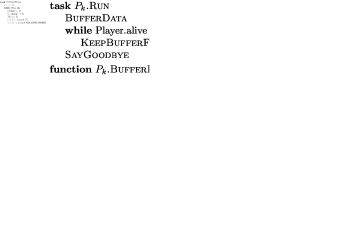
\includegraphics[width=0.75\textwidth]{chunk_generation_and_flooding}
  \fig{500}{5cm}{DBS_splitter_feed} \caption{Chunk
    generation at the splitter and their transmission to the
    team.\label{fig:chunk_generation}}
\end{figure*}
\end{comment}

We define a \emph{round} as the process of transmitting $N$ different
chunks from the splitter to a team of $N$ peers. In other words, for a
team of size $N$, the round-time is $N$ chunk-times. Notice that the
round-time is variable, and depends on the current number of peers in
the team ($N$), the chunk size ($C$), and the average bit-rate of the
media stream.

The splitter remembers which chunk, of a list of the last $B$
transmitted chunks, was sent to each peer of the team. Notice that, in
order to remember in a round which chunk was sent to each peer, $B\ge
N$. \note{See \href{https://github.com/P2PSP/simulator/blob/f0c73be1817e7d3b816cc61cd2c8e59b17f9a0e6/src/core/splitter_dbs.py\#L296}{$\text{destination\_of\_chunk}[]$ in \texttt{splitter\_dbs.py}}.}

\begin{comment}
(in a team) as the time necessary to send two consecutive chunks from
  the splitter (of such team) to the same peer, using the
  round-robing. This time is variable and depends on $|T|$, $C$, and
  the average bit-rate of the media, $A$.
\end{comment}

\begin{comment}
The round-time is defined by:
\begin{equation}
  \cal{r} = \cal{c}N.
  \label{eq:round_time}
\end{equation}
For example, if we use only one team of $N=256$ peers, a chunk size
$C=1024$~bytes, and a video of $1$~Mb/s, the round time is
\begin{displaymath}
  \cal{r} = \frac{1024\frac{\text{bytes}}{\text{chunk}}\times
    8\frac{\text{bits}}{\text{byte}}}{10^6\frac{\text{bits}}{\text{second}}}\times
  256 \approx 2.1~\text{seconds}.
\end{displaymath}
\end{comment}
